\chapter{Introduction to Multi-task Robot Control and Planning}
Unlike an industrial robot which usually execute specific tasks in a static environment, service robots face a much more complex and dynamic situation. These uncertainties and complexity required service robots to deal with multiple tasks simultaneously.
\begin{figure}
\centering
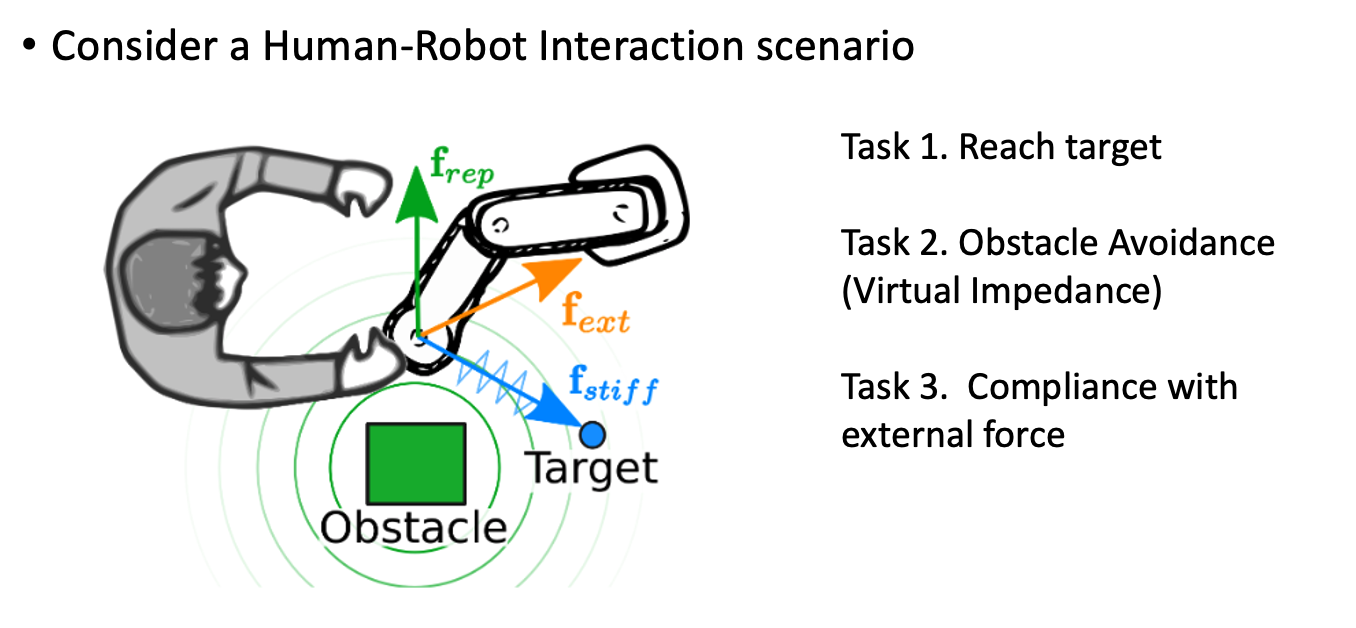
\includegraphics[width=0.55\textwidth]{images/motivation_scenario.png}
\caption{A Human-Robot interaction scenario}
\label{fig:Human-Robot interaction scenario}
\end{figure}

As Figure ~\ref{fig:Human-Robot interaction scenario} shows, a robot in this HRI scenario may have three tasks. Firstly, the robot needs to reach the target pose. Secondly, no collision is allowed to happened during the entire process (\textit{Collision Avoidance}). Lastly, to meet the safety consideration, the robot should compliance with external force imposed by humans (\textit{Compliance Control}).
 
As we can imagine, It is impossible for a robot to complete these three tasks perfectly in the same time. Either in the task space or in the configuration space, the limited variables with greater number of constraints usually return no solution. 

%ToDo citations here
A naive idea is to sum up the dynamics behavior ~\cite{Santis:2007:ASME}, but this simple idea may lead to an unstable problem, the equilibrium point is undetermined in most  cases. For example, the final pose of the robot may actually collide with obstacles.
One of the common approaches to this multi-tasks problem is null-space projection. In two tasks situation, this method isolate the first task from the second one. By treating each task in a different priority, the method project the second priority task  into the null-space of Jacobian related to the first one. 
For example, when both goal reaching and collision avoidance is considered, the \textit{task-first} type concept will place the  original robot control task in a higher priority, 
while use only the null space of Jacobian to prevent the robot from collisions. There are several problems behind this idea, it needs the robot to be highly redundant with 
respect to the task. But we can hardly find whether the null space related to original task is large enough to avoid obstacles. 
On the contrary, the \textit{avoidance-first} type approach let the original control scheme only operates in the null space of Jacobian related to collision avoidance. 
To meet safety demand in multi-priority problem, collision avoidance behavior should be set to the top priority, hence it is usually more considerable than the previous one. 
When it comes to cases where more than two tasks to be dealt with, many null-space projection based architectures were proposed to systematically handle with these tasks.
%ToDo nullspace projection method formulae
\begin{equation}
\qdd = {\Jb}^{\dagger} (\xdd - \Jd\qd)+ \mathbf{N} \qdd_0 
\end{equation}
let $\tilde{\xdd} = \xdd - \Jd\qd$
Where $\mathbf{N} = (\Ib - {\Jb}^{\dagger} \Jb)$

Many other articles  addressed  this by applying optimization based approaches. Among them, Quatratic Programming (QP) is a common choice which formulize a quaduatic math optimization 
problem by a quaduatic cost function subjected to serveral linear constraints. In the context, we may want to treat the original task as the main task, so it should be 
expressed in the cost function 
\begin{equation}
f(\qdd) = \| \Jb\qdd  - \xdd + \Jd\qd\|^2
\end{equation}
and find the $\qd = argmin_\qdd'\|\Jb\qdd' - \xdd + \Jd\qd  \|^2$ as the optimal  in no constraint cases. 

